\subsection{Basics of Electronics}

In this section, we'll have a look at fundamental things of electronics.  We'll also point you to the right references to understand the concept in an easy way. I think that the best way to really grasp what this is all about is through water analogies. Because we see water every day (as opposed to electrons), it is a lot easier to understand elementary fluid dynamics concepts than elementary electricity concepts. Fortunately, whoever created this world loved the concept of \textit{Fractals} and self-similar patterns, so it's very easy \footnote{Honestly it's almost scary how similar it is, you'd believe it's all the same thing. This makes me thing of a slightly unrelated essay which thinks about a (to me) similar epistemological problem: https://en.wikipedia.org/wiki/The_Unreasonable\_Effectiveness\_of\_Mathematics\_in\_the\_Natural\_Sciences} to make accurate electricity analogies with water.  
Because this course is goes in depth into electronics, it is assumed that all these concepts are already fairly familiar to the student. I have chosen to cover it just as a reminder or merely a pointer to what one should know before starting the course. I really believe that if one is not fully comfortably with these concepts, time should \textit{first} be spent understanding them before going further into the course. Most of these things are quite straightforward and should not take to a graduate student with a scientific background more than a day to grasp. It is not needed to enter deep theory into each of these concepts, but one should clearly be familiar enough with them. 

\subsubsection{Charge}

Electric charge is the physical property of matter that causes it to experience a force when placed in an electromagnetic field. Electric charge can be positive or negative (commonly carried by protons and electrons respectively). Alike charges repel each other and unlike charges attract each other. An object with an absence of net charge is referred to as neutral. We define charge with the symbol $Q$ and with the units of \textit{Coulombs}. 

\subsubsection{Electric Field}

An electric field is the physical field that surrounds electrically-charged particles and exerts force on all other charged particles in the field, either attracting or repelling them. It also refers to the physical field for a system of charged particles. Electric field is important, and actually not so obvious to grasp. It would take me quite some time to explain it well, I recommend having a look at the \textit{Khan Academy} \footnote{https://www.khanacademy.org/science/hs-physics/x215e29cb31244fa1:types-of-interactions/x215e29cb31244fa1:electric-and-magnetic-fields/v/electric-field-definition} explanation as I won't be able to do anything better than this. 

\subsubsection{Voltage}

Voltage\footnote{Section mostly copy-pasted from: https://www.electronics-tutorials.ws/dccircuits/dcp\_1.html}, ($V$) is the potential energy of an electrical supply stored in the form of an electrical charge. Voltage can be thought of as the force that pushes electrons through a conductor and the greater the voltage the greater is its ability to “push” the electrons through a given circuit. As energy has the ability to do work this potential energy can be described as the work required in joules to move electrons in the form of an electrical current around a circuit from one point or node to another.

Then the difference in voltage between any two points, connections or junctions (called nodes) in a circuit is known as the Potential Difference, (p.d.) commonly called the Voltage Drop.

The Potential difference between two points is measured in Volts with the circuit symbol V, or lowercase “v“, although Energy, E lowercase “e” is sometimes used to indicate a generated emf (electromotive force). Then the greater the voltage, the greater is the pressure (or pushing force) and the greater is the capacity to do work.

A constant voltage source is called a DC Voltage with a voltage that varies periodically with time is called an AC voltage. Voltage is measured in volts, with one volt being defined as the electrical pressure required to force an electrical current of one ampere through a resistance of one Ohm. 

Batteries or power supplies are mostly used to produce a steady D.C. (direct current) voltage source such as 5v, 12v, 24v etc in electronic circuits and systems. While A.C. (alternating current) voltage sources are available for domestic house and industrial power and lighting as well as power transmission.

\textbf{Voltage is always measured as the difference between any two points in a circuit and the voltage between these two points is generally referred to as the “Voltage drop“}. Note that voltage can exist across a circuit without current, but current cannot exist without voltage and as such any voltage source whether DC or AC likes an open or semi-open circuit condition but hates any short circuit condition as this can destroy it.

\begin{figure}[H]
    \centering
    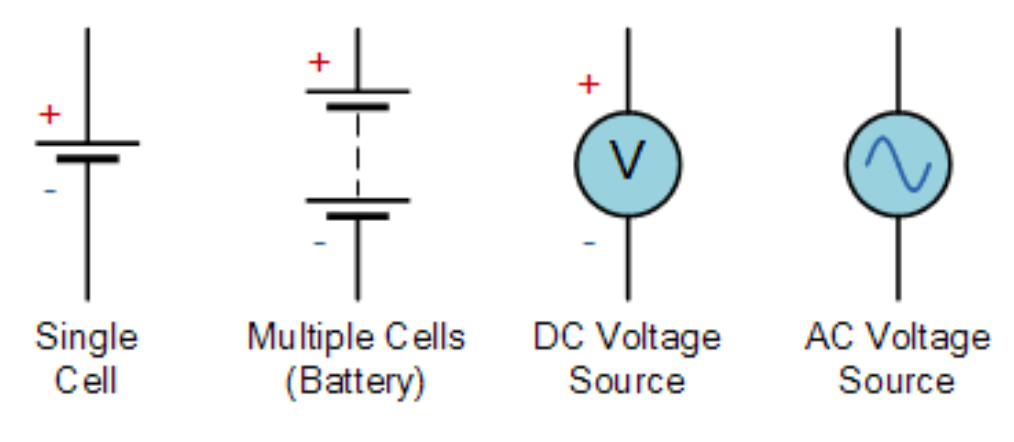
\includegraphics[width=0.65\linewidth]{../../Figures/Voltage.PNG}
    \caption{Voltage. Adapted from https://www.electronics-tutorials.ws/dccircuits/dcp\_1.html}
    \label{fig:Resistors}
\end{figure}

\subsubsection{Current}

Electrical Current \footnote{Section mostly copy-pasted from: https://www.electronics-tutorials.ws/dccircuits/dcp\_1.html}, ($I$) is the movement or flow of electrical charge and is measured in Amperes, symbol i, for intensity). It is the continuous and uniform flow (called a drift) of electrons (the negative particles of an atom) around a circuit that are being “pushed” by the voltage source. In reality, electrons flow from the negative (–ve) terminal to the positive (+ve) terminal of the supply and for ease of circuit understanding conventional current flow assumes that the current flows from the positive to the negative terminal.

Generally in circuit diagrams the flow of current through the circuit usually has an arrow associated with the symbol, $I$, or lowercase i to indicate the actual direction of the current flow. However, this arrow usually indicates the direction of conventional current flow and not the direction of the actual flow. This is because of Benjamin Franklin: \textit{"As far as the history goes, Ben Franklin imagined electricity as a type of invisible fluid that could build up or be absent from a material, or at least certain materials. He believed that when this invisible fluid built up the object was positively charged. When there was an absence of this fluid he called that material negatively charged. It turns out he got the concept right but the nomenclature backwards."}. So it really is because of him that conventional current flow is not in the same direction as electron flow. Once you get used to it it's fine, but this can be quite annoying sometimes when you're trying to visualize things. 

\begin{figure}[H]
    \centering
    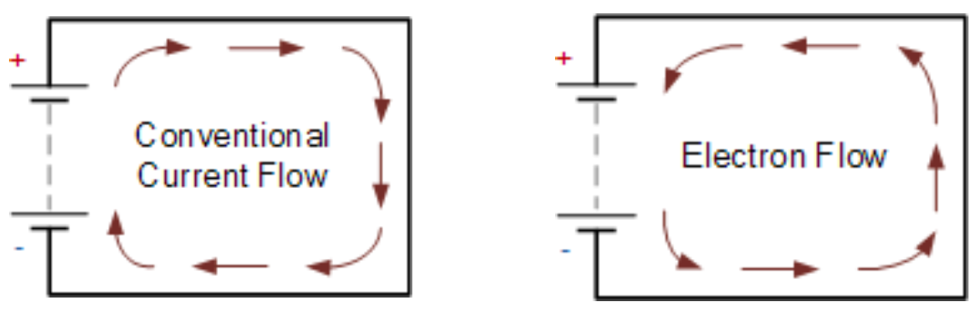
\includegraphics[width=0.65\linewidth]{../../Figures/Electron_Flow.PNG}
    \caption{Electron flow and conventional current. Adapted from https://www.electronics-tutorials.ws/dccircuits/dcp\_1.html}
    \label{fig:Resistors}
\end{figure}

\subsubsection{Resistance}

\begin{figure}[H]
    \centering
    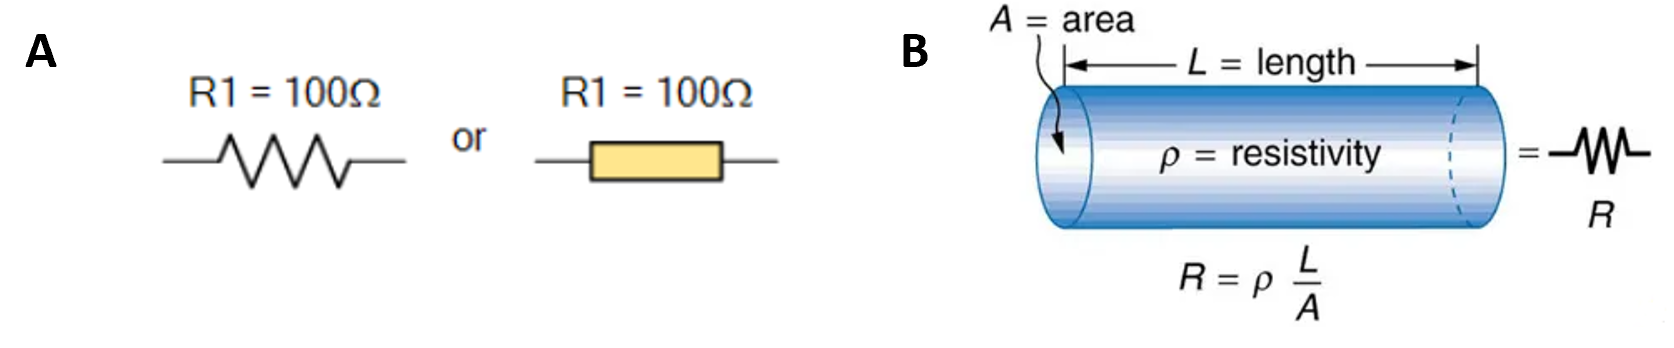
\includegraphics[width=0.65\linewidth]{../../Figures/Resistors.PNG}
    \caption{Resistor electric symbols. Adapted from https://www.electronics-tutorials.ws/resistor/res\_1.html}
    \label{fig:Resistors}
\end{figure}

The principal job of a resistor\footnote{Section mostly copy-pasted from: https://www.electronics-tutorials.ws/resistor/res\_1.html} within an electrical circuit is to “resist” (hence the name Resistor), regulate or to set the flow of electrons (current) through them by using the type of conductive material from which they are composed. Resistors can also be connected together in various series and parallel combinations to form resistor networks which can act as voltage droppers, voltage dividers or current limiters within a circuit.

Resistors are represented in electrical circuits as shown in figure \ref{fig:Resistors}.A and resistance is measured in \textit{Ohms} ($\ohm$). They are called “Passive Devices”, because they contain no source of power or amplification but only attenuate or reduce the voltage or current signal passing through them. This attenuation results in electrical energy being lost in the form of heat as the resistor resists the flow of electrons through it.

Then a potential difference is required between the two terminals of a resistor for current to flow. This potential difference balances out the energy lost. When used in DC circuits the potential difference, also known as a resistors voltage drop, is measured across the terminals as the circuit current flows through the resistor.

Most types of resistor are linear devices that produce a \textit{voltage drop} across themselves when an electrical current flows through them because they obey \textit{Ohm’s Law} (more on that in the next section), and different values of resistance produces different values of current or voltage. This can be very useful in Electronic circuits by controlling or reducing either the current flow or voltage produced across them we can produce a voltage-to-current and current-to-voltage converter.

The resistance of any substance depends on the following factors: 1) the length of the device ($L$), 2) the cross sectional area of the device ($A$), 3) the nature of material of the device, which has an inherent \textit{resistivity} ($\rho$, measured in $\ohm.m$), 4) the temperature of the device ($T$) (see Figure \ref{fig:Resistors}.B). 

\begin{equation}
    R = \rho \frac{L}{A}
\end{equation}

We say that a physical element or device has \textbf{infinite resistance} when current doesn't flow through it: it is an \textbf{insulator}.\footnote{We actually say infinite impedance but I haven't introduced impedance yet so bear with me. Also, there is always a tiny tiny bit of current flowing, but is negligible. That's why the concept of \textit{infinite} impedance is only theoretical: all insulators can become conductors if we apply a strong enough voltage. This will be covered substantially more in the device physics section in chapter 2.}

\subsubsection{Ohm's law}

Simply, there is a linear relationship that relates Voltage and Current: 
\begin{equation}
    I = \frac{V}{R}
\end{equation}

\subsubsection{DC vs AC and exponential notation}

The explanations dealt with so far have constant voltage sources and are just take at steady state. Once the current is established, it is thus also a constant. Direct current (DC) is the flow of electric charge in only one direction. It is the steady state of a constant-voltage circuit. Most well-known applications, however, use a time-varying voltage source, and time varying signals in general. This is relevant here not because we consider AC per se but rather because we consider charging and discharging properties of some circuits that have capacitance - on which the time component needs to be considered. Alternating current (AC) is the flow of electric charge that periodically reverses direction. If the source varies periodically, particularly sinusoidally, the circuit is known as an alternating current circuit. Examples include the commercial and residential power that serves so many of our needs. Figure 1 shows graphs of voltage and current versus time for typical DC and AC power. The AC voltages and frequencies commonly used in homes and businesses vary around the world. 

\begin{figure}[H]
    \centering
    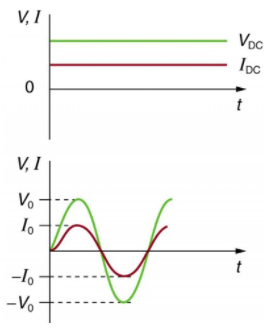
\includegraphics[width=0.35\linewidth]{../../Figures/ACDC.PNG}
    \caption{Alternating and direct current. Adapted from \url{https://courses.lumenlearning.com/physics/chapter/20-5-alternating-current-versus-direct-current/}}
    \label{fig:ACDC}
\end{figure}

If we're dealing with a different type of signal, we must use a different type of notation and consider the differences with DC. As can be seen on Figure \ref{fig:ACDC}, AC behaves in waves, so it is appropriate to treat is as such and use relevant notation that describes it properly. Also, we will be using conventional notation for time varying voltage $u(t)$ and current $i(t)$ (as opposed to V and I that were previously used). We can now define:  


\begin{equation}
    u(t) = U\mathrm{cos}(\omega t + \phi) = Ue^{j\omega t + \phi}\footnote{This is derived from Euler's formula: $e^{jx} = \mathrm{cos}(x) + j\mathrm{sin}(x)$}
\end{equation}

Where $U$ is the amplitude (peak value) of voltage, $\omega$ is the angular frequency, $\phi$ is the phase offset (more on the phase in a second).


\paragraph{Impedance}

There is a generalization of resistance, called \textit{impedance} (represented by the symbol $Z$). It is also measured in Ohms. It is not really useful when working with DC current, but takes meaning when working with AC current, which has a complex component to it (which we call reactance but no one cares really). \textbf{Ohm's law still applies in AC} and impedance is simply the ratio of the complex (wave) representation of sinusoidal voltage ($u(t)$) between its terminals to the complex (wave) representation of the current ($i(t)$) flowing through it. This means that Ohm's law still applies!  Impedance therefore possesses both magnitude and phase; resistance, on the other hand, has magnitude but no phase. This is why we say that impedance is a generalization of resistance, as resistance is only a special case of impedance. For impedence, we note: 

\begin{equation}
    Z = R + jX
\end{equation}

where R is the real part resistance and the imaginary part X is the reactance. The magnitude of $Z$ is $|Z| = \sqrt{R^2 + X^2}$, while the phase is $\phi = \mathrm{arctan}(\frac{X}{R})$. In general, $\phi$ is the phase difference between alternating voltage and current: $\phi = \phi_v - \phi_i$ 


\subsubsection{Capacitance}

\begin{figure}[H]
    \centering
    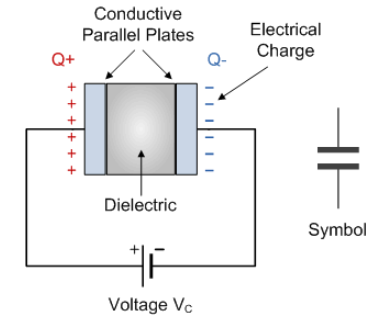
\includegraphics[width=0.55\linewidth]{../../Figures/Capacitors.PNG}
    \caption{Capacitor structure and electric symbol. Adapted from https://www.electronics-tutorials.ws/capacitor/cap_1.html}
    \label{fig:Capacitors}
\end{figure}

The capacitor\footnote{Section mostly copy-pasted from: https://www.electronics-tutorials.ws/capacitor/cap_1.html} is a component which has the ability or “capacity” to store energy in the form of an electrical charge producing a potential difference (Static Voltage) across its plates, much like a small rechargeable battery.
Capacitance is the electrical property of a capacitor and is the measure of a capacitors ability to store an electrical charge onto its two plates with the unit of capacitance being the Farad (abbreviated to F) named after the British physicist Michael Faraday
There are many different kinds of capacitors available from very small capacitor beads used in resonance circuits to large power factor correction capacitors, but they all do the same thing, they store charge.
In its basic form, a capacitor consists of two or more parallel conductive (metal) plates which are not connected or touching each other, but are electrically separated either by air or by some form of a good insulating material such as waxed paper, mica, ceramic, plastic or some form of a liquid gel as used in electrolytic capacitors. The insulating layer between a capacitors plates is commonly called the Dielectric.
Due to this insulating layer, DC current can not flow through the capacitor as it blocks it allowing instead a voltage to be present across the plates in the form of an electrical charge.

Also, because capacitors store the energy of the electrons in the form of an electrical charge on the plates the larger the plates and/or smaller their separation the greater will be the charge that the capacitor holds for any given voltage across its plates. In other words, larger plates, smaller distance, more capacitance. This yields the following relation:

\begin{equation}
    C = \frac{\epsilon_0 A}{d}
\end{equation}

with $C$ capacitance in Farads ($F$), $\epsilon$ permittivity of the dielectric \footnote{Permittivity is a measure of the electric \textit{polarizability} of a dielectric. A material with high permittivity polarizes more in response to an applied electric field than a material with low permittivity, thereby storing more energy in the material}, $A$ area of the plate overlap in $m^2$ and $d$ distance between the plates in meter. 

By applying a voltage to a capacitor and measuring the charge on the plates, the ratio of the charge Q (in Coulomns) to the voltage V (in Volts) will give the capacitance value of the capacitor and is therefore given by the following important relation: 
\begin{equation*}
    C = \frac{Q}{V}
\end{equation*}

Although the charge is stored on the plates of a capacitor, it is more exact to say that the energy within the charge is stored in an “electrostatic field” between the two plates. When an electric current flows into the capacitor, it charges up, so the electrostatic field becomes much stronger as it stores more energy between the plates.

Likewise, as the current flowing out of the capacitor, discharging it, the potential difference between the two plates decreases and the electrostatic field decreases as the energy moves out of the plates.

\textbf{Still not sure you understand?} If you feel like you still need to grasp the fundamental idea behind a capacitor, go watch the brilliant video by \textit{The Engineering Mindset} on capacitors \footnote{https://www.youtube.com/watch?v=X4EUwTwZ110}.

\paragraph{Capacitance in complex analysis}
Capacitance is most often studied with complex analysis, so let's do that here and apply it to Ohm's law. While the current flowing through a resistor is given by the voltage applied to it, the current that flows through a capacitor is proportional to the voltage change. 

\begin{equation}
    i(t) = \frac{dQ}{dt} = \frac{d(C V)}{dt} = C\frac{du(t)}{dt}
\end{equation}

Here, $i(t)$ is the current through time, which we defined previously as being the derivative of charge Q with respect to time. We also previously defined Q as being equal to the capacitance times voltage V (following from $C = Q/V$). By convention, we most often note voltage through time as $u$ or $u(t)$ instead of $V$. Same for current, which we note as $i(t)$ instead of $I$.

Differentiation can be conveniently performed in complex notation, yielding the following: 

\begin{equation}
    \frac{du(t)}{dt} = \frac{d (Ue^{j\omega t)}}{dt} = j\omega U e^{jwt} = j\omega u(t) 
\end{equation}

Therefore, for a capacitor, $i(t) = C\frac{du(t)}{dt} = j\omega \cdot C \cdot u(t)$



\subsubsection{Water analogies}


\subsubsection{Basics of Parallel and Series circuits}

\begin{figure}[H]
    \centering
    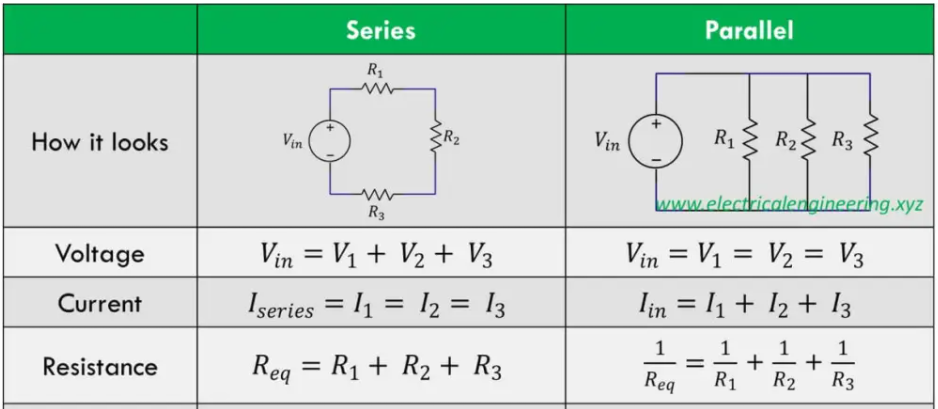
\includegraphics[width=0.75\linewidth]{../../Figures/Parallel_Series.PNG}
    \caption{Parallel and Series circuit comparison. Adapted from \url{https://www.electricalengineering.xyz/questions/top-5-differences-between-series-and-parallel-circuits/}}
    \label{fig:Parallel_Series}
\end{figure}

When dealing with electronic circuits, you can plug things in a variety of different ways, and some key things are to remember. Figure \ref{fig:Parallel_S} does a great job at explaining this. Voltage drops across devices connected in series, but it is conserved across different branches of a circuit. Current is just the opposite (which make sense when you think of water flow): it divides when separated into different branches and is maintained when flowing around a single loop. Resistance adds itself in series, which means that connecting two resistors together in the same branch makes the overall resistance stronger. This doesn't apply in parallel, where another relation need to be applied to find the total resistance of the circuit. Capacitance, which is not shown on the figure, is actually exactly the opposite of resistance, it adds up in parallel and follows the same principle as resistance in parallel when it is connected in series. 

\subsubsection{Kirchoff's Voltage and Current Laws}

One very important law is needed to understand many circuits we'll be studying: Kirchoff's law. 

\begin{itemize}
    \item Current law: All current flowing into a node (or junction) must be equal to the current flowing out of it. This means that there is no charge (think water) disappearing.
    \begin{equation}
        \sum I_{in} = \sum I_{in}
    \end{equation}
    \item Voltage law: In any complete loop within a circuit, the sum of all voltages across components which supply electrical energy (such as cells or generators) must equal the sum of all voltages across the other components in the same loop. This law is a consequence of both charge conservation and the conservation of energy.
    \begin{equation}
        \sum V_{total} = 0
    \end{equation}
\end{itemize}

The following figure\footnote{Adapted from: https://www.sciencefacts.net/kirchhoffs-law.html} makes this much easier to understand.  

\begin{figure}[H]
    \centering
    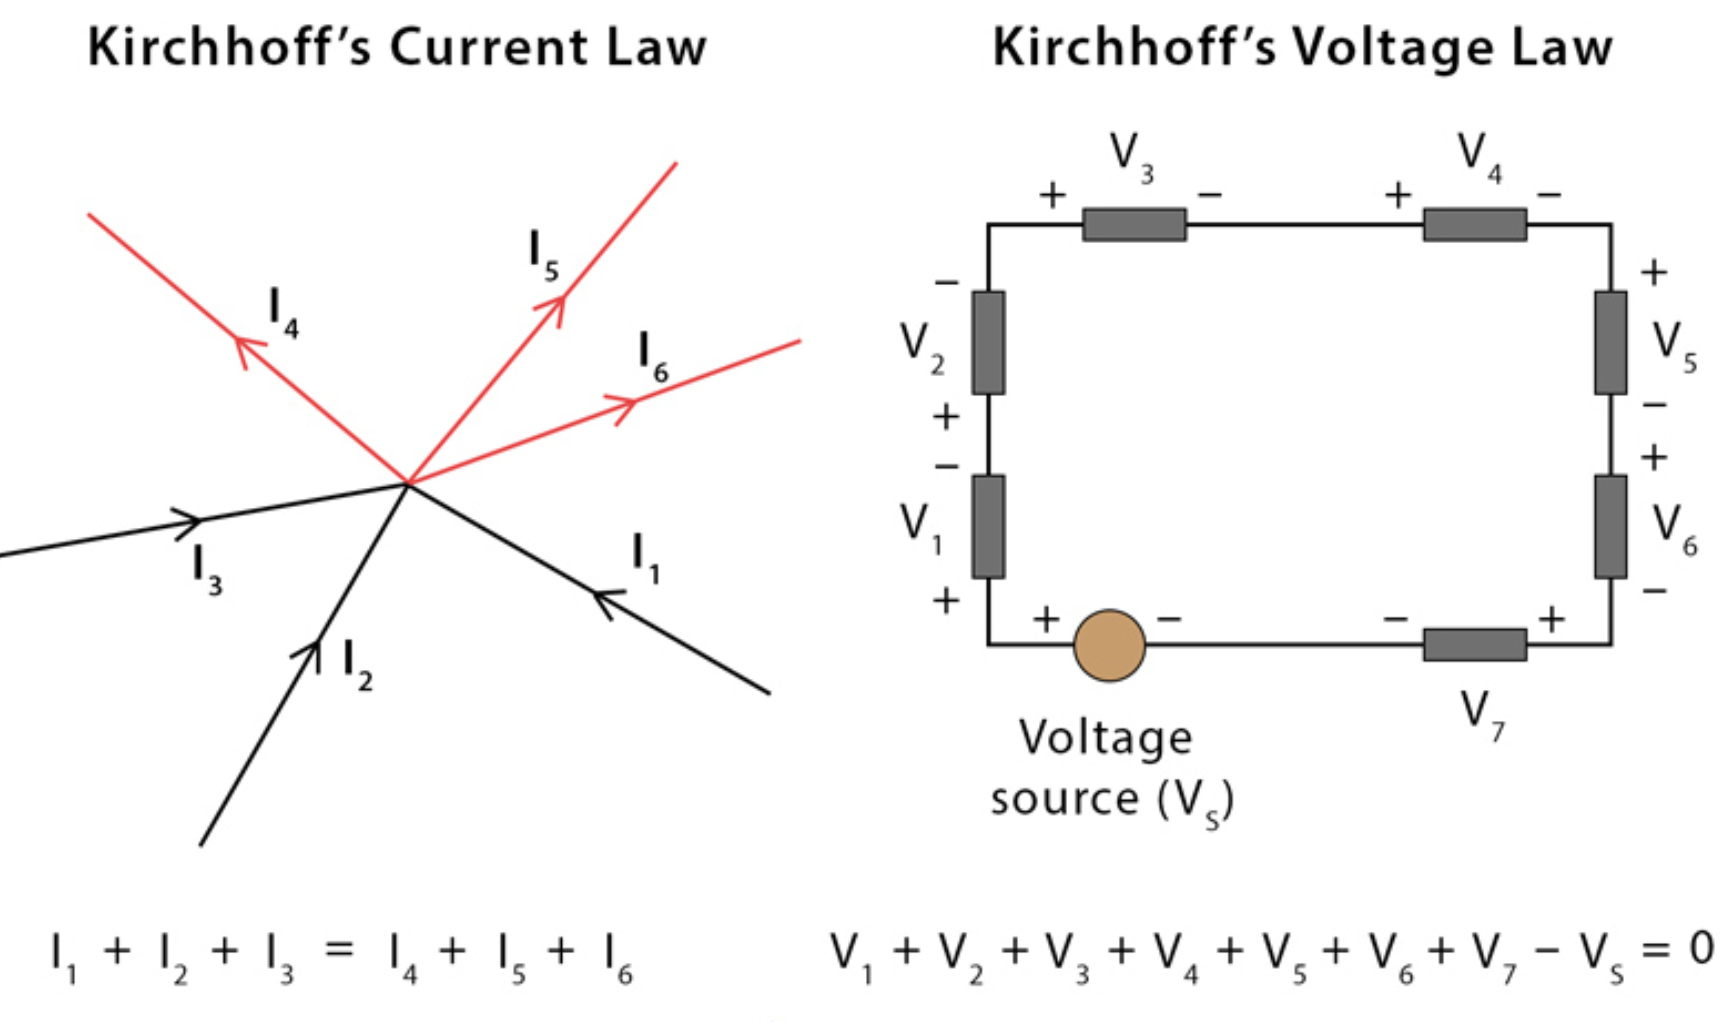
\includegraphics[width=0.6\linewidth]{../../Figures/Kirchoff.PNG}
    \caption{Kirchoff's current and voltage laws. Adapted from https://www.electronics-tutorials.ws/capacitor/cap_1.html}
    \label{fig:Capacitors}
\end{figure}




